\documentclass{standalone}
\usepackage{tikz}
\usetikzlibrary{patterns, positioning}
\usepackage[sfdefault]{ClearSans} %% option 'sfdefault' activates Clear Sans as the default text font
\usepackage[T1]{fontenc}

\begin{document}
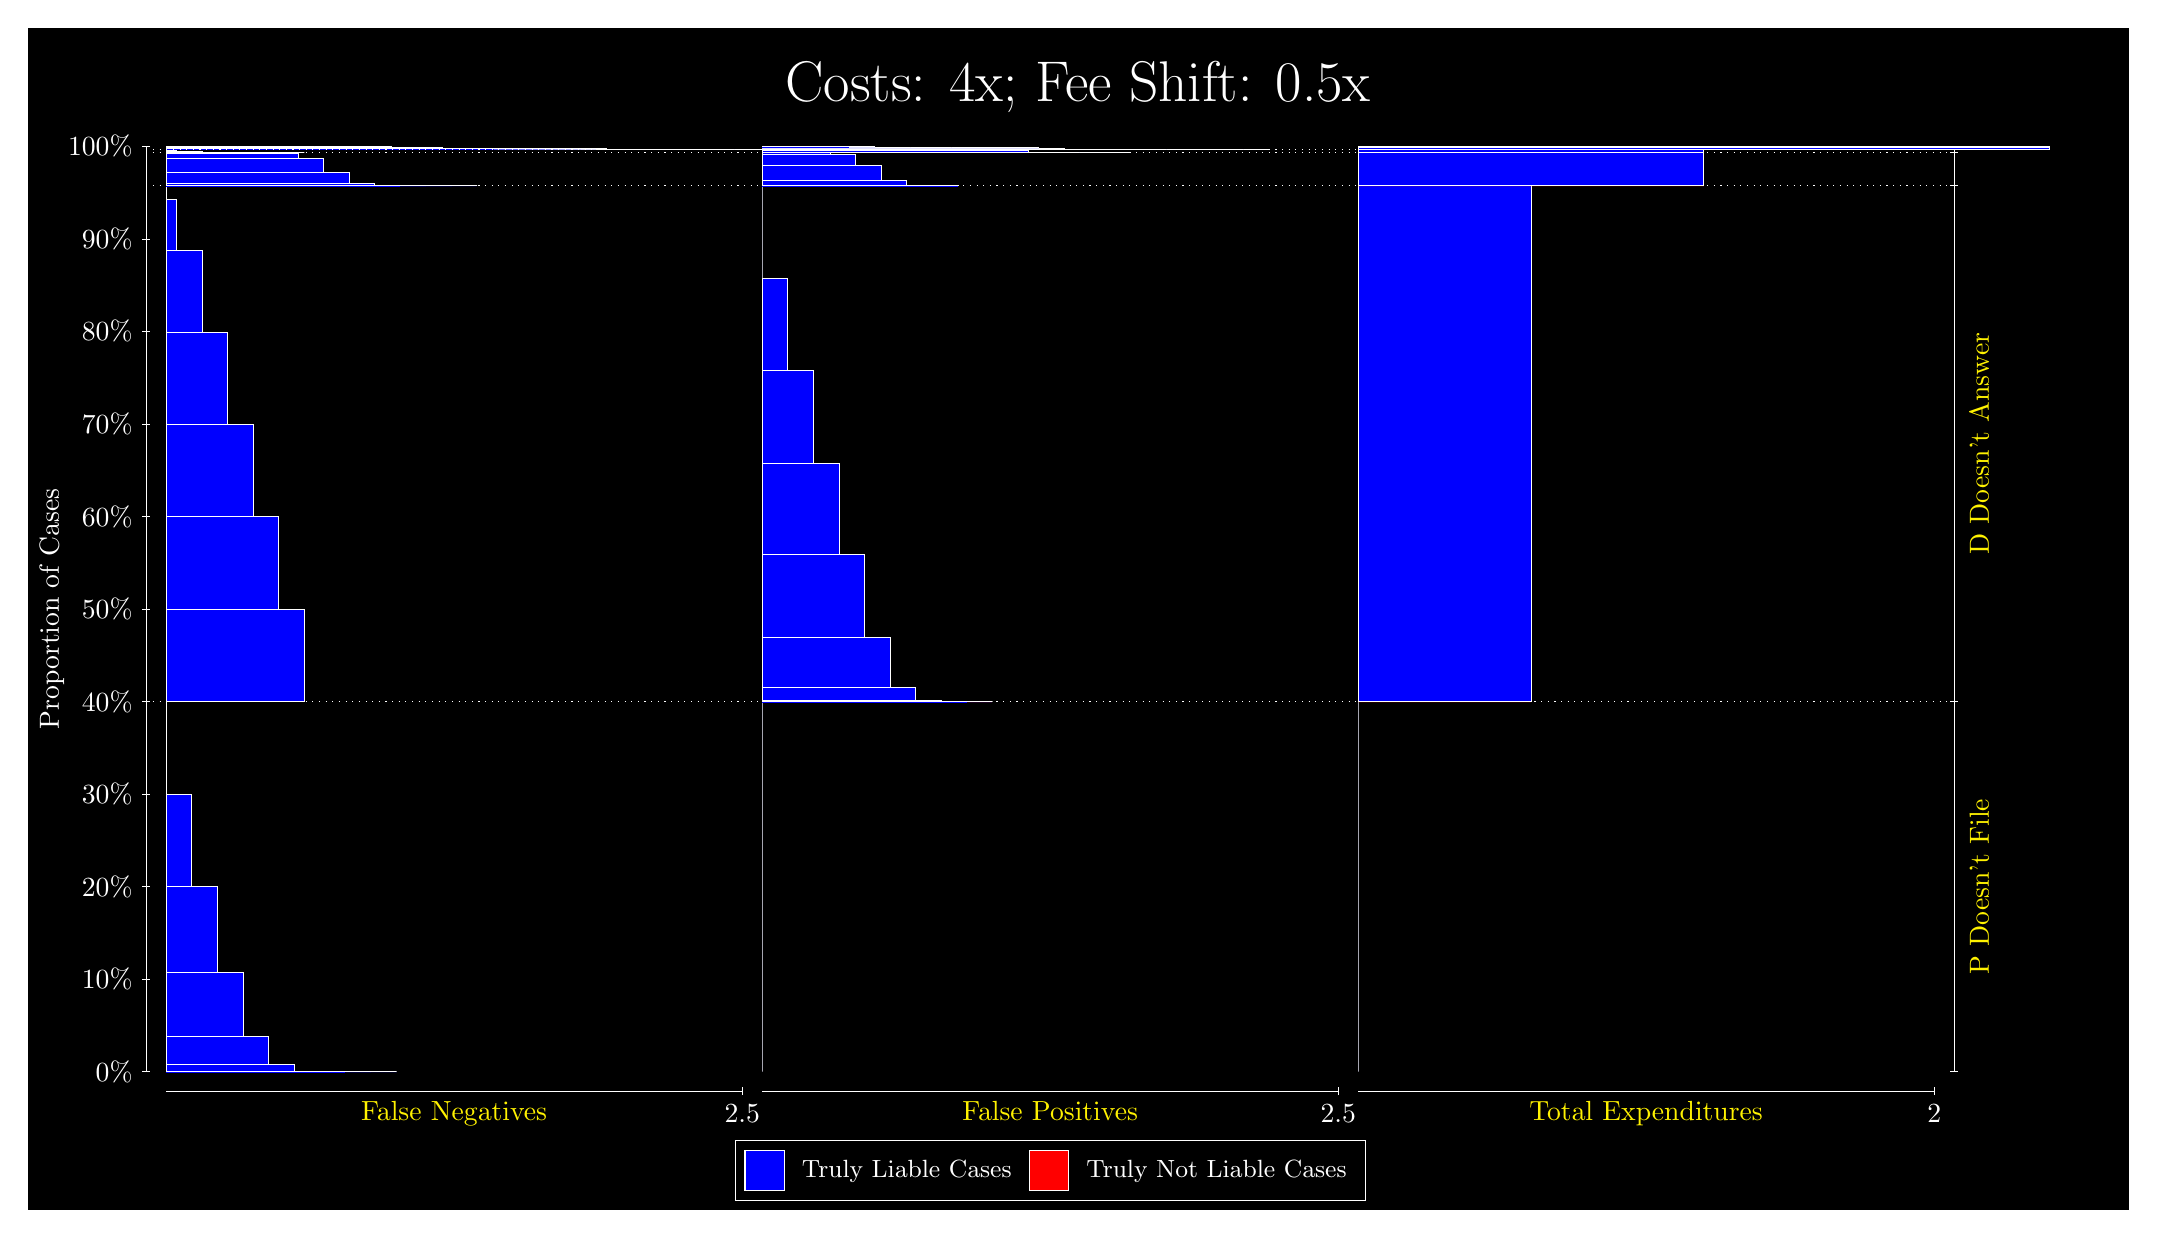
\begin{tikzpicture}
\draw[fill=black] (0,0) rectangle (26.667,15);
\draw[text=white] (0,13.5) rectangle (26.667,15) node[midway] {\huge Costs: 4x; Fee Shift: 0.5x};
\draw[white, very thin] (1.5,1.75) -- (1.5,13.5);
\node[rotate=90, text=white, anchor=center] at (0.3, 7.625) {Proportion of Cases};
\draw[white, very thin] (1.45,1.75) -- (1.55,1.75);
\node[text=white, anchor=east] at (1.45, 1.75) {0\%};
\draw[white, very thin] (1.45,2.925) -- (1.55,2.925);
\node[text=white, anchor=east] at (1.45, 2.925) {10\%};
\draw[white, very thin] (1.45,4.1) -- (1.55,4.1);
\node[text=white, anchor=east] at (1.45, 4.1) {20\%};
\draw[white, very thin] (1.45,5.275) -- (1.55,5.275);
\node[text=white, anchor=east] at (1.45, 5.275) {30\%};
\draw[white, very thin] (1.45,6.45) -- (1.55,6.45);
\node[text=white, anchor=east] at (1.45, 6.45) {40\%};
\draw[white, very thin] (1.45,7.625) -- (1.55,7.625);
\node[text=white, anchor=east] at (1.45, 7.625) {50\%};
\draw[white, very thin] (1.45,8.8) -- (1.55,8.8);
\node[text=white, anchor=east] at (1.45, 8.8) {60\%};
\draw[white, very thin] (1.45,9.975) -- (1.55,9.975);
\node[text=white, anchor=east] at (1.45, 9.975) {70\%};
\draw[white, very thin] (1.45,11.15) -- (1.55,11.15);
\node[text=white, anchor=east] at (1.45, 11.15) {80\%};
\draw[white, very thin] (1.45,12.325) -- (1.55,12.325);
\node[text=white, anchor=east] at (1.45, 12.325) {90\%};
\draw[white, very thin] (1.45,13.5) -- (1.55,13.5);
\node[text=white, anchor=east] at (1.45, 13.5) {100\%};

\draw[white, very thin] (24.457,1.75) -- (24.457,13.5);
\draw[white, very thin] (24.407,1.75) -- (24.507,1.75);
\node[anchor=west] at (24.407, 1.75) {};
\draw[white, very thin] (24.407,6.4468) -- (24.507,6.4468);
\node[anchor=west] at (24.407, 6.4468) {};
\draw[white, very thin] (24.407,13.001) -- (24.507,13.001);
\node[anchor=west] at (24.407, 13.001) {};
\draw[white, very thin] (24.407,13.423) -- (24.507,13.423);
\node[anchor=west] at (24.407, 13.423) {};
\draw[white, very thin] (24.407,13.461) -- (24.507,13.461);
\node[anchor=west] at (24.407, 13.461) {};
\draw[white, very thin] (24.407,13.5) -- (24.507,13.5);
\node[anchor=west] at (24.407, 13.5) {};

\draw[white, very thin, fill=blue] (1.75,1.75) rectangle (4.6775,1.75);
\draw[white, very thin, fill=blue] (1.75,1.75) rectangle (4.3523,1.75);
\draw[white, very thin, fill=blue] (1.75,1.75) rectangle (4.027,1.7503);
\draw[white, very thin, fill=blue] (1.75,1.7503) rectangle (3.7017,1.7576);
\draw[white, very thin, fill=blue] (1.75,1.7576) rectangle (3.3764,1.836);
\draw[white, very thin, fill=blue] (1.75,1.836) rectangle (3.0511,2.198);
\draw[white, very thin, fill=blue] (1.75,2.198) rectangle (2.7258,3.0096);
\draw[white, very thin, fill=blue] (1.75,3.0096) rectangle (2.4006,4.1052);
\draw[white, very thin, fill=blue] (1.75,4.1052) rectangle (2.0753,5.2722);
\draw[white, very thin, fill=red] (1.75,5.2722) rectangle (1.75,5.2722);
\draw[white, very thin, fill=blue] (1.75,5.2722) rectangle (1.75,6.4468);
\draw[white, very thin, fill=blue] (1.75,6.4468) rectangle (3.5065,7.6218);
\draw[white, very thin, fill=blue] (1.75,7.6218) rectangle (3.1812,8.7968);
\draw[white, very thin, fill=blue] (1.75,8.7968) rectangle (2.856,9.9714);
\draw[white, very thin, fill=blue] (1.75,9.9714) rectangle (2.5307,11.135);
\draw[white, very thin, fill=blue] (1.75,11.135) rectangle (2.2054,12.184);
\draw[white, very thin, fill=blue] (1.75,12.184) rectangle (1.8801,12.822);
\draw[white, very thin, fill=red] (1.75,12.822) rectangle (1.75,12.822);
\draw[white, very thin, fill=blue] (1.75,12.822) rectangle (1.75,13.001);
\draw[white, very thin, fill=blue] (1.75,13.001) rectangle (5.7022,13.001);
\draw[white, very thin, fill=blue] (1.75,13.001) rectangle (5.3769,13.001);
\draw[white, very thin, fill=blue] (1.75,13.001) rectangle (5.0516,13.001);
\draw[white, very thin, fill=blue] (1.75,13.001) rectangle (4.7263,13.002);
\draw[white, very thin, fill=blue] (1.75,13.002) rectangle (4.4011,13.029);
\draw[white, very thin, fill=blue] (1.75,13.029) rectangle (4.0758,13.168);
\draw[white, very thin, fill=blue] (1.75,13.168) rectangle (3.7505,13.35);
\draw[white, very thin, fill=blue] (1.75,13.35) rectangle (3.4252,13.415);
\draw[white, very thin, fill=blue] (1.75,13.415) rectangle (3.0999,13.423);
\draw[white, very thin, fill=blue] (1.75,13.423) rectangle (2.7746,13.423);
\draw[white, very thin, fill=red] (1.75,13.423) rectangle (1.75,13.423);
\draw[white, very thin, fill=blue] (1.75,13.423) rectangle (3.5065,13.423);
\draw[white, very thin, fill=blue] (1.75,13.423) rectangle (3.1812,13.423);
\draw[white, very thin, fill=blue] (1.75,13.423) rectangle (2.856,13.423);
\draw[white, very thin, fill=blue] (1.75,13.423) rectangle (2.5307,13.426);
\draw[white, very thin, fill=blue] (1.75,13.426) rectangle (2.2054,13.439);
\draw[white, very thin, fill=blue] (1.75,13.439) rectangle (1.8801,13.456);
\draw[white, very thin, fill=red] (1.75,13.456) rectangle (1.75,13.456);
\draw[white, very thin, fill=blue] (1.75,13.456) rectangle (1.75,13.461);
\draw[white, very thin, fill=blue] (1.75,13.461) rectangle (9.9471,13.461);
\draw[white, very thin, fill=blue] (1.75,13.461) rectangle (9.6218,13.461);
\draw[white, very thin, fill=blue] (1.75,13.461) rectangle (9.2966,13.461);
\draw[white, very thin, fill=blue] (1.75,13.461) rectangle (8.9713,13.461);
\draw[white, very thin, fill=blue] (1.75,13.461) rectangle (8.646,13.461);
\draw[white, very thin, fill=blue] (1.75,13.461) rectangle (8.3207,13.462);
\draw[white, very thin, fill=blue] (1.75,13.462) rectangle (8.3207,13.462);
\draw[white, very thin, fill=blue] (1.75,13.462) rectangle (7.9954,13.462);
\draw[white, very thin, fill=blue] (1.75,13.462) rectangle (7.9954,13.463);
\draw[white, very thin, fill=blue] (1.75,13.463) rectangle (7.6702,13.466);
\draw[white, very thin, fill=blue] (1.75,13.466) rectangle (7.3449,13.467);
\draw[white, very thin, fill=blue] (1.75,13.467) rectangle (7.3449,13.469);
\draw[white, very thin, fill=blue] (1.75,13.469) rectangle (7.2148,13.469);
\draw[white, very thin, fill=blue] (1.75,13.469) rectangle (7.0196,13.469);
\draw[white, very thin, fill=blue] (1.75,13.469) rectangle (6.8895,13.469);
\draw[white, very thin, fill=blue] (1.75,13.469) rectangle (6.6943,13.469);
\draw[white, very thin, fill=blue] (1.75,13.469) rectangle (6.5642,13.469);
\draw[white, very thin, fill=blue] (1.75,13.469) rectangle (6.369,13.469);
\draw[white, very thin, fill=blue] (1.75,13.469) rectangle (6.2389,13.469);
\draw[white, very thin, fill=blue] (1.75,13.469) rectangle (5.9136,13.47);
\draw[white, very thin, fill=blue] (1.75,13.47) rectangle (5.9136,13.47);
\draw[white, very thin, fill=blue] (1.75,13.47) rectangle (5.5883,13.476);
\draw[white, very thin, fill=blue] (1.75,13.476) rectangle (5.5883,13.476);
\draw[white, very thin, fill=blue] (1.75,13.476) rectangle (5.2631,13.486);
\draw[white, very thin, fill=blue] (1.75,13.486) rectangle (4.9378,13.488);
\draw[white, very thin, fill=blue] (1.75,13.488) rectangle (4.9378,13.494);
\draw[white, very thin, fill=blue] (1.75,13.494) rectangle (4.6125,13.494);
\draw[white, very thin, fill=blue] (1.75,13.494) rectangle (4.6125,13.497);
\draw[white, very thin, fill=blue] (1.75,13.497) rectangle (4.6125,13.498);
\draw[white, very thin, fill=blue] (1.75,13.498) rectangle (4.2872,13.499);
\draw[white, very thin, fill=blue] (1.75,13.499) rectangle (4.2872,13.5);
\draw[white, very thin, fill=blue] (1.75,13.5) rectangle (3.9619,13.5);
\draw[white, very thin, fill=blue] (1.75,13.5) rectangle (3.6366,13.5);
\draw[white, very thin, fill=blue] (1.75,13.5) rectangle (3.3114,13.5);
\draw[white, very thin, fill=blue] (1.75,13.5) rectangle (3.3114,13.5);
\draw[white, very thin, fill=blue] (1.75,13.5) rectangle (2.9861,13.5);
\draw[white, very thin, fill=blue] (1.75,13.5) rectangle (2.9861,13.5);
\draw[white, very thin, fill=blue] (1.75,13.5) rectangle (2.6608,13.5);
\draw[white, very thin, fill=blue] (1.75,13.5) rectangle (2.6608,13.5);
\draw[white, very thin, fill=blue] (1.75,13.5) rectangle (2.3355,13.5);
\draw[white, very thin, fill=red] (1.75,13.5) rectangle (1.75,13.5);
\draw[white, very thin, fill=red] (9.3189,1.75) rectangle (9.3189,1.75);
\draw[white, very thin, fill=blue] (9.3189,1.75) rectangle (9.3189,6.4468);
\draw[white, very thin, fill=red] (9.3189,6.4468) rectangle (12.246,6.4468);
\draw[white, very thin, fill=blue] (9.3189,6.4468) rectangle (12.246,6.4468);
\draw[white, very thin, fill=blue] (9.3189,6.4468) rectangle (11.921,6.4471);
\draw[white, very thin, fill=blue] (9.3189,6.4471) rectangle (11.596,6.4599);
\draw[white, very thin, fill=blue] (9.3189,6.4599) rectangle (11.271,6.6261);
\draw[white, very thin, fill=blue] (9.3189,6.6261) rectangle (10.945,7.2645);
\draw[white, very thin, fill=blue] (9.3189,7.2645) rectangle (10.62,8.3136);
\draw[white, very thin, fill=blue] (9.3189,8.3136) rectangle (10.295,9.4768);
\draw[white, very thin, fill=blue] (9.3189,9.4768) rectangle (9.9694,10.651);
\draw[white, very thin, fill=blue] (9.3189,10.651) rectangle (9.6442,11.826);
\draw[white, very thin, fill=blue] (9.3189,11.826) rectangle (9.3189,13.001);
\draw[white, very thin, fill=red] (9.3189,13.001) rectangle (11.807,13.001);
\draw[white, very thin, fill=blue] (9.3189,13.001) rectangle (11.807,13.002);
\draw[white, very thin, fill=blue] (9.3189,13.002) rectangle (11.482,13.009);
\draw[white, very thin, fill=blue] (9.3189,13.009) rectangle (11.157,13.074);
\draw[white, very thin, fill=blue] (9.3189,13.074) rectangle (10.831,13.256);
\draw[white, very thin, fill=blue] (9.3189,13.256) rectangle (10.506,13.396);
\draw[white, very thin, fill=blue] (9.3189,13.396) rectangle (10.181,13.422);
\draw[white, very thin, fill=blue] (9.3189,13.422) rectangle (9.8556,13.423);
\draw[white, very thin, fill=blue] (9.3189,13.423) rectangle (9.5303,13.423);
\draw[white, very thin, fill=blue] (9.3189,13.423) rectangle (9.3189,13.423);
\draw[white, very thin, fill=red] (9.3189,13.423) rectangle (14.003,13.423);
\draw[white, very thin, fill=blue] (9.3189,13.423) rectangle (14.003,13.423);
\draw[white, very thin, fill=blue] (9.3189,13.423) rectangle (13.678,13.423);
\draw[white, very thin, fill=blue] (9.3189,13.423) rectangle (13.352,13.423);
\draw[white, very thin, fill=blue] (9.3189,13.423) rectangle (13.027,13.428);
\draw[white, very thin, fill=blue] (9.3189,13.428) rectangle (12.702,13.446);
\draw[white, very thin, fill=blue] (9.3189,13.446) rectangle (12.377,13.459);
\draw[white, very thin, fill=blue] (9.3189,13.459) rectangle (12.051,13.461);
\draw[white, very thin, fill=blue] (9.3189,13.461) rectangle (11.726,13.461);
\draw[white, very thin, fill=blue] (9.3189,13.461) rectangle (11.401,13.461);
\draw[white, very thin, fill=blue] (9.3189,13.461) rectangle (11.075,13.461);
\draw[white, very thin, fill=red] (9.3189,13.461) rectangle (15.759,13.461);
\draw[white, very thin, fill=blue] (9.3189,13.461) rectangle (15.759,13.461);
\draw[white, very thin, fill=blue] (9.3189,13.461) rectangle (15.434,13.461);
\draw[white, very thin, fill=red] (9.3189,13.461) rectangle (15.434,13.461);
\draw[white, very thin, fill=blue] (9.3189,13.461) rectangle (15.434,13.461);
\draw[white, very thin, fill=red] (9.3189,13.461) rectangle (15.109,13.461);
\draw[white, very thin, fill=blue] (9.3189,13.461) rectangle (15.109,13.461);
\draw[white, very thin, fill=blue] (9.3189,13.461) rectangle (15.109,13.461);
\draw[white, very thin, fill=blue] (9.3189,13.461) rectangle (14.784,13.461);
\draw[white, very thin, fill=red] (9.3189,13.461) rectangle (14.784,13.461);
\draw[white, very thin, fill=blue] (9.3189,13.461) rectangle (14.784,13.461);
\draw[white, very thin, fill=blue] (9.3189,13.461) rectangle (14.784,13.461);
\draw[white, very thin, fill=blue] (9.3189,13.461) rectangle (14.458,13.461);
\draw[white, very thin, fill=red] (9.3189,13.461) rectangle (14.458,13.461);
\draw[white, very thin, fill=blue] (9.3189,13.461) rectangle (14.458,13.461);
\draw[white, very thin, fill=blue] (9.3189,13.461) rectangle (14.458,13.461);
\draw[white, very thin, fill=blue] (9.3189,13.461) rectangle (14.133,13.462);
\draw[white, very thin, fill=red] (9.3189,13.462) rectangle (14.133,13.462);
\draw[white, very thin, fill=blue] (9.3189,13.462) rectangle (14.133,13.462);
\draw[white, very thin, fill=blue] (9.3189,13.462) rectangle (14.133,13.462);
\draw[white, very thin, fill=blue] (9.3189,13.462) rectangle (13.808,13.462);
\draw[white, very thin, fill=blue] (9.3189,13.462) rectangle (13.808,13.463);
\draw[white, very thin, fill=red] (9.3189,13.463) rectangle (13.808,13.463);
\draw[white, very thin, fill=blue] (9.3189,13.463) rectangle (13.808,13.463);
\draw[white, very thin, fill=blue] (9.3189,13.463) rectangle (13.808,13.463);
\draw[white, very thin, fill=blue] (9.3189,13.463) rectangle (13.482,13.463);
\draw[white, very thin, fill=blue] (9.3189,13.463) rectangle (13.482,13.467);
\draw[white, very thin, fill=blue] (9.3189,13.467) rectangle (13.482,13.467);
\draw[white, very thin, fill=blue] (9.3189,13.467) rectangle (13.157,13.468);
\draw[white, very thin, fill=blue] (9.3189,13.468) rectangle (13.157,13.475);
\draw[white, very thin, fill=blue] (9.3189,13.475) rectangle (13.157,13.476);
\draw[white, very thin, fill=blue] (9.3189,13.476) rectangle (12.832,13.476);
\draw[white, very thin, fill=blue] (9.3189,13.476) rectangle (12.832,13.485);
\draw[white, very thin, fill=blue] (9.3189,13.485) rectangle (12.832,13.485);
\draw[white, very thin, fill=blue] (9.3189,13.485) rectangle (12.507,13.486);
\draw[white, very thin, fill=blue] (9.3189,13.486) rectangle (12.507,13.491);
\draw[white, very thin, fill=blue] (9.3189,13.491) rectangle (12.507,13.491);
\draw[white, very thin, fill=blue] (9.3189,13.491) rectangle (12.181,13.491);
\draw[white, very thin, fill=blue] (9.3189,13.491) rectangle (12.181,13.491);
\draw[white, very thin, fill=blue] (9.3189,13.491) rectangle (12.181,13.492);
\draw[white, very thin, fill=blue] (9.3189,13.492) rectangle (11.856,13.492);
\draw[white, very thin, fill=blue] (9.3189,13.492) rectangle (11.856,13.492);
\draw[white, very thin, fill=red] (9.3189,13.492) rectangle (11.726,13.492);
\draw[white, very thin, fill=blue] (9.3189,13.492) rectangle (11.726,13.492);
\draw[white, very thin, fill=blue] (9.3189,13.492) rectangle (11.531,13.492);
\draw[white, very thin, fill=blue] (9.3189,13.492) rectangle (11.531,13.492);
\draw[white, very thin, fill=red] (9.3189,13.492) rectangle (11.401,13.492);
\draw[white, very thin, fill=blue] (9.3189,13.492) rectangle (11.401,13.492);
\draw[white, very thin, fill=blue] (9.3189,13.492) rectangle (11.206,13.492);
\draw[white, very thin, fill=red] (9.3189,13.492) rectangle (11.075,13.492);
\draw[white, very thin, fill=blue] (9.3189,13.492) rectangle (11.075,13.492);
\draw[white, very thin, fill=blue] (9.3189,13.492) rectangle (11.075,13.493);
\draw[white, very thin, fill=blue] (9.3189,13.493) rectangle (10.88,13.493);
\draw[white, very thin, fill=blue] (9.3189,13.493) rectangle (10.75,13.495);
\draw[white, very thin, fill=blue] (9.3189,13.495) rectangle (10.75,13.495);
\draw[white, very thin, fill=blue] (9.3189,13.495) rectangle (10.425,13.497);
\draw[white, very thin, fill=blue] (9.3189,13.497) rectangle (10.425,13.498);
\draw[white, very thin, fill=blue] (9.3189,13.498) rectangle (10.1,13.499);
\draw[white, very thin, fill=blue] (9.3189,13.499) rectangle (10.1,13.5);
\draw[white, very thin, fill=blue] (9.3189,13.5) rectangle (9.7743,13.5);
\draw[white, very thin, fill=blue] (9.3189,13.5) rectangle (9.7743,13.5);
\draw[white, very thin, fill=blue] (9.3189,13.5) rectangle (9.449,13.5);
\draw[white, very thin, fill=blue] (9.3189,13.5) rectangle (9.3189,13.5);
\draw[white, very thin, fill=red] (16.888,1.75) rectangle (16.888,1.75);
\draw[white, very thin, fill=blue] (16.888,1.75) rectangle (16.888,6.4468);
\draw[white, very thin, fill=red] (16.888,6.4468) rectangle (19.083,6.4468);
\draw[white, very thin, fill=blue] (16.888,6.4468) rectangle (19.083,13.001);
\draw[white, very thin, fill=red] (16.888,13.001) rectangle (21.279,13.001);
\draw[white, very thin, fill=blue] (16.888,13.001) rectangle (21.279,13.423);
\draw[white, very thin, fill=red] (16.888,13.423) rectangle (21.279,13.423);
\draw[white, very thin, fill=blue] (16.888,13.423) rectangle (21.279,13.461);
\draw[white, very thin, fill=red] (16.888,13.461) rectangle (25.67,13.461);
\draw[white, very thin, fill=blue] (16.888,13.461) rectangle (25.67,13.461);
\draw[white, very thin, fill=red] (16.888,13.461) rectangle (25.67,13.461);
\draw[white, very thin, fill=blue] (16.888,13.461) rectangle (25.67,13.492);
\draw[white, very thin, fill=red] (16.888,13.492) rectangle (25.67,13.492);
\draw[white, very thin, fill=blue] (16.888,13.492) rectangle (25.67,13.5);
\draw[white, dotted] (1.5,6.4468) -- (24.457,6.4468);
\draw[white, dotted] (1.5,13.001) -- (24.457,13.001);
\draw[white, dotted] (1.5,13.423) -- (24.457,13.423);
\draw[white, dotted] (1.5,13.461) -- (24.457,13.461);
\draw[white, very thin] (1.75,1.5) -- (9.0689,1.5);
\node[text=yellow, anchor=north] at (5.4094, 1.5) {False Negatives};
\draw[white, very thin] (9.0689,1.45) -- (9.0689,1.55);
\node[text=white, anchor=north] at (9.0689, 1.45) {2.5};

\draw[white, very thin] (9.3189,1.5) -- (16.638,1.5);
\node[text=yellow, anchor=north] at (12.978, 1.5) {False Positives};
\draw[white, very thin] (16.638,1.45) -- (16.638,1.55);
\node[text=white, anchor=north] at (16.638, 1.45) {2.5};

\draw[white, very thin] (16.888,1.5) -- (24.207,1.5);
\node[text=yellow, anchor=north] at (20.547, 1.5) {Total Expenditures};
\draw[white, very thin] (24.207,1.45) -- (24.207,1.55);
\node[text=white, anchor=north] at (24.207, 1.45) {2};

\node[text=yellow, centered, rotate=90] at (24.777, 4.0984) {P Doesn't File};
\node[text=yellow, centered, rotate=90] at (24.777, 9.7241) {D Doesn't Answer};




\draw (12.978300999999998,1.5) node[draw=none] (baseCoordinate) {};
\begin{scope}[align=center]
        \matrix[scale=0.5, draw=white, below=0.5cm of baseCoordinate, nodes={draw}, column sep=0.1cm]{
            \node[rectangle, draw, minimum width=0.5cm, minimum height=0.5cm, fill=blue] {}; &
            \node[draw=none, font=\small, text=white] (B) {Truly Liable Cases}; &
            \node[rectangle, draw, minimum width=0.5cm, minimum height=0.5cm, fill=red] {}; &
            \node[draw=none, font=\small, text=white] (B) {Truly Not Liable Cases}; \\
            };
\end{scope}

\end{tikzpicture}
\end{document}